\documentclass[11pt]{article}
\usepackage[review]{acl}
\usepackage{times}
\usepackage{latexsym}
\usepackage[utf8]{inputenc}
\usepackage{microtype}
\usepackage{amssymb}
\usepackage{microtype}
\usepackage{inconsolata}
\usepackage{graphicx}
\usepackage{listings}
\usepackage{xcolor}
\usepackage[T1]{fontenc}
\usepackage{float}
\usepackage{booktabs}
\usepackage{tikz}
\usetikzlibrary{positioning}
\IfFileExists{inconsolata.sty}
{\usepackage{inconsolata}}{}
\usepackage{amsmath}
\usepackage{booktabs}
\usepackage{tcolorbox}
\tcbuselibrary{breakable,skins}

\usepackage{pgfplots}
\pgfplotsset{compat=1.18}
\usepackage{subcaption}

\newtcolorbox{promptbox}{
  breakable,
  colback=gray!8,
  colframe=gray!55,
  boxrule=0.4pt,
  arc=1pt,
  left=6pt, right=6pt, top=5pt, bottom=5pt,
  fontupper=\small\raggedright,
  before skip=6pt, after skip=6pt
}

\title{LLMs Annotating Sentiment Spans with Reliable Offsets: A Eight-Model Pipeline Study}
\author{Anonymous ACL Submission}

\begin{document}
\maketitle
\begin{abstract}
% Structured sentiment annotation requires models to identify opinions and locate their spans in the source text. These requirements can fail independently: a plausible opinion may have unusable offsets, while an aligned span may express the wrong meaning. We study a pipeline that asks models to select indexed tokens, constructs character offsets deterministically, and validates outputs with corrective retries. Seven instruction-tuned models annotate 763 Portuguese hotel reviews in SSA and ASQP formats under three configurations. Indexed tokens with retries retain more annotations than either direct-offset generation or token selection without retries in all 16 model--task pairs. Full-pipeline rejection ranges from 0.6\% to 94.3\% for SSA and 0.4\% to 95.6\% for ASQP. All retained non-null spans align with their source substrings, conditional on validation. Retries increase retention but reduce measured annotation throughput. A partial human audit identifies semantic errors despite valid offsets. The study distinguishes structural reliability and annotation productivity from semantic adequacy, which requires separate assessment.
\end{abstract}

\section{Introduction}
Data annotation aims at labeling unlabeled data to fit a specific machine learning task or statistical analysis. In the domain of Sentiment Analysis~\cite{Liu_2012}, two sub-tasks have emerged with specific data structures requiring annotation expertise: Aspect-Sentiment Quad Prediction (ASQP)~\cite{asqp_original} and Structured Sentiment Analysis (SSA)~\cite{barnes-2021-ssa-dependency}.

Given an opinion \textit{O} emitted by holder \textit{H} towards a target \textit{T} of category \textit{C} with sentiment expression \textit{E} and polarity \textit{P}, ASQP and SSA extract tuples as \textit{(C, T, E, P)} and \textit{(H, T, E, P)}, respectively. An example of labeling in both tasks is shown in Figure~\ref{fig:tasks_fig}. Each task demands fine-grained annotation, which increases the complexity of the process, since labels are not simply categorical (e.g., 0 or 1), which can slow down the annotation process~\cite{tan2024largelanguagemodelsdata}. We refer to ``target`` and ``aspect`` interchangeable.


Both tasks are commonly addressed with encoder-based strategies \cite{asqp_original, barnes-2021-ssa-dependency} that require offset information for each word to employ BIO tagging, where B marks a span's first token, I its continuation, and O tokens outside any span, as in Named Entity Recognition. In this context, annotation complexity gains a new factor, since simply marking the words does not guarantee that the semantic structure of the opinion is preserved. For example, consider the opinion \textit{Great coffee, but the room was small and dirty. Despite the good coffee, we'll not come back.} Since \textit{coffee} appears twice, it is important to ensure that the offset associated with \textit{coffee} in the tuple \textit{(food, coffee, great, POS)} correctly refers to the first occurrence, so that the intended semantics is preserved.

Despite recent advances of Large Language Models (LLMs) across several tasks, we empirically observe that LLMs struggle to produce reliable offsets for the spans they label. To address this problem, we propose a simple, yet effective, offset-aware strategy that indexes each token in a sentence and has the model select spans by token ID instead of generating raw character positions. This strategy drastically reduces the rejection rate relative to direct offset generation, although it does not by itself guarantee the semantic adequacy of the retained annotations, which we assess separately through a human evaluation.

\definecolor{posgreen}{HTML}{0F6E56}
\definecolor{negred}{HTML}{C32D2D}
\definecolor{allyellow}{HTML}{B27B00} % Amarelo/âmbar escuro para boa legibilidade

\newcommand{\aspect}[4]{%
  % #1 = cor da borda/fundo do span, #2 = texto do span, #3 = cor da etiqueta, #4 = texto da etiqueta
  \tikz[baseline=(n.base)]{%
    \node[inner xsep=2pt, inner ysep=4pt, rounded corners=2pt,
          draw=#1, line width=0.8pt, fill=#1!8]
      (n) {\strut #2};
    \node[above=1pt of n, inner sep=.5pt, text=#3, font=\scriptsize] {#4};%
  }%
}

\begin{figure}[t]
  \centering
  \setlength{\fboxsep}{0pt}
  \begin{minipage}{\columnwidth}
    \raggedright
    \small
    \vspace{3.5ex}
    % Exemplo ASQP: (category, target, expression, polarity)
    O \aspect{posgreen}{café da manhã}{posgreen}{\textbf{food} / positive} era ótimo,
    mas o \aspect{negred}{quarto}{negred}{\textbf{rooms} / negative} estava sujo.

    \smallskip\smallskip


    \textit{\color{gray!50!black} The breakfast was great, but the room was dirty.}

    \vspace{3.5ex}
    % Exemplo SSA: (holder, target, expression, polarity)
    % Holder em amarelo, expressão em vermelho e target/polaridade em verde
    \aspect{allyellow}{Eu}{allyellow}{holder} \aspect{negred}{odeio}{negred}{expression} quando o \aspect{posgreen}{atendimento}{posgreen}{target (+)} demora tanto.

    \smallskip\smallskip
    \textit{\color{gray!50!black} I hate when the service takes so long.}
  \end{minipage}
  \caption{ASQP and SSA examples.}
  \label{fig:tasks_fig}
\end{figure}

\section{Related Work}
LLMs have demonstrated strong annotation capabilities in both zero-shot \cite{zeroshot} and few-shot \cite{fewshotlearn} settings. Early work revealed that ChatGPT performed surprisingly well on hate speech detection \cite{gpths}, while GPT-3 was evaluated across four NLP annotation tasks by \cite{ding-etal-2023-gpt}, establishing a foundation for subsequent research in LLM-based annotation.

More recently, \cite{Bojic2025} conducted a large-scale comparison of eight LLMs — including GPT-4 and Llama 3.1-70B — against 33 human annotators on sentiment analysis and political leaning classification, finding that model performance approached human-level agreement. However, the integration of LLMs into annotation pipelines is not without risks. \cite{schroeder-etal-2025-just} found that AI-generated annotation suggestions introduced anchoring bias in human annotators without yielding any time savings, raising concerns about the suitability of human-AI collaborative annotation. Furthermore, adversarial prompts have been shown to systematically fool LLMs into producing incorrect annotations \cite{AlaofiFooled}.

At the span level, \cite{kasner-etal-2026-llms} employed DeepSeek R1 70B and GPT-4o as span annotators, achieving high inter-annotator agreement with human raters. In the domain of structured data, \cite{zhang-etal-2025-tablellm} reported over 80\% accuracy on tabular data generation using GPT-4o and TableLLM, suggesting that LLMs may be particularly well-suited for annotation tasks involving structured or semi-structured inputs.

\section{Method}
\subsection{Data and tasks}
We use two Brazilian Portuguese TripAdvisor datasets, each containing 763 reviews. SSA provides 3,438 reference tuples linking holder, aspect, opinion expression, and polarity; ASQP provides 3,436 tuples linking category, aspect, expression, and polarity. The six categories are structure, service, location, general, price, and others; polarities are POS, NEG, and NEU. Reviews are directly annotated, without paraphrasing or showing their reference responses to the model.

\subsection{Tokenization and span selection}
The pipeline first splits each review into sentences using punctuation rules and a fixed abbreviation list, producing 3,831 processing units per task. It then identifies each sequence of non-whitespace characters as a token. Tokens receive consecutive IDs starting at zero, together with their start and end positions in the unchanged sentence. This is a simple text index, separate from the language model's own tokenizer.

For example, \textit{O quarto era muito bom.} becomes \texttt{0: O}, \texttt{1: quarto}, \texttt{2: era}, \texttt{3: muito}, and \texttt{4: bom.} The model receives the sentence and the indexed token list. To annotate the room as the target and \textit{muito bom.} as the opinion, it selects ID 1 for the aspect and IDs 3--4 for the expression. Its JSON response also contains the copied terms, polarity, and the task-specific holder or category.

Code converts the selected IDs into character offsets. It takes the start of the first selected token and the end of the last, then adds the sentence's starting position in the review. In the example, the aspect occupies $[2,8)$ and the expression $[13,23)$ relative to the sentence. The start is inclusive and the end exclusive. Spans are recovered from the original text, preserving any internal spacing. This lets the model choose the text while the pipeline computes its location.

\subsection{Validation and retries}
The validator checks the JSON structure, permitted labels, and selected spans. Token IDs must exist and be ordered, unique, and contiguous; each reported term must match the corresponding source substring. An absent SSA holder uses a null term and an empty span. The pipeline does not search nearby text to repair boundaries.

When validation fails, the model receives its previous response and feedback describing the errors. Full allows up to three retries after the initial request. A valid response ends the loop; a unit that still fails is discarded. Empty annotation lists can pass validation and are counted separately. Task-specific guides explain the annotation conventions and output format (Appendix~\ref{app:prompts}).

\subsection{Models and configurations}
We run eight models: Qwen2.5-Instruct at 0.5B, 1.5B, 3B, and 7B; Gemma 3 at 4B and 12B; Qwen3.8-27B; and Gemma 4 31B. Gemma 3 uses the public Unsloth BF16 repositories; Qwen3.8 and Gemma 4 use their official Qwen and Google repositories in BF16 without quantization.

Each model performs both tasks under three conditions, giving 48 runs. Full combines indexed tokens with retries. $-$tokens asks for sentence-relative character offsets directly, keeping retries. $-$retry keeps indexed tokens but allows only one request per unit. Segmentation, semantic instructions, and validation remain fixed; guides and demonstrations use the span format required by each condition.

We serve models with vLLM, one per GPU, with 200 concurrent client requests and an 8,192-token context limit. Generation uses temperature 0, top-$p=0.8$, top-$k=20$, presence penalty 1.0, and at most 768 output tokens; requests set \texttt{enable\_thinking=False}. Each run saves document predictions, processing metadata, and a dataset checksum in JSON.

\subsection{Validation and retries}
The validator checks the JSON structure, permitted labels, and selected spans. Token IDs must exist and be ordered, unique, and contiguous; each reported term must match the corresponding source substring. An absent holder uses a null term and an empty span. The pipeline does not search nearby text to repair boundaries.

When validation fails, the model receives its previous response and feedback describing the errors. Full allows up to three retries after the initial request. A valid response ends the loop; a unit that still fails is discarded. Empty annotation lists can pass validation and are counted separately. Task-specific guides and four fixed synthetic demonstrations explain the annotation conventions and output format (Appendix~\ref{app:prompts}).

\begin{table*}[!t]
\centering\small
\renewcommand{\arraystretch}{1.08}
\setlength{\tabcolsep}{6pt}
\begin{tabular}{lrrr@{\hskip 16pt}rrr}
\toprule
& \multicolumn{3}{c}{\textbf{SSA}} & \multicolumn{3}{c}{\textbf{ASQP}} \\
\cmidrule(lr){2-4}\cmidrule(lr){5-7}
Model & Rejc. (\%) & Tuples & Empty & Rejc. (\%) & Tuples & Empty \\
\midrule
Qwen2.5-0.5B & 94.3 & 219 & 0 & 95.6 & 173 & 2 \\
Qwen2.5-1.5B & 67.0 & 1,760 & 5 & 58.2 & 1,869 & 83 \\
Qwen2.5-3B & 42.1 & 1,909 & 900 & 27.7 & 2,132 & 1,167 \\
Qwen2.5-7B & 42.2 & 2,546 & 373 & 34.5 & 2,642 & 426 \\
Gemma 3 4B & 46.8 & 1,969 & 641 & 58.9 & 1,707 & 338 \\
Gemma 3 12B & 6.6 & 5,790 & 359 & 4.6 & 5,755 & 251 \\
Qwen3.8-27B & 0.6 & 5,494 & 874 & 0.4 & 5,774 & 717 \\
Gemma 4 31B & 1.6 & 6,340 & 519 & 0.4 & 6,423 & 468 \\
\bottomrule
\end{tabular}
\caption{Full pipeline for eight models. Each task contains 763 documents and 3,831 sentence units. Empty denotes accepted outputs without annotations.}
\label{tab:full}
\end{table*}

\section{Results}

Rejection tends to decrease as model size increases, though not monotonically within a family.

\noindent\textbf{SSA.} Qwen2.5-0.5B rejects the most units by a wide margin (94.3\%), retaining only 219 tuples. Scaling to Qwen2.5-1.5B substantially reduces rejection to 67.0\%, raising yield to 1,760 tuples. At 3B and 7B, the trend is not monotonic: Qwen2.5-3B rejects 42.1\% of units, essentially matching Qwen2.5-7B's 42.2\%, despite the latter retaining more tuples overall (2,546 versus 1,909). Gemma 3 follows a comparable pattern at a smaller scale: Gemma 3 4B rejects 46.8\% of units, close to the mid-sized Qwen2.5 models, while Gemma 3 12B drops sharply to 6.6\%, retaining 5,790 tuples. At the largest scale, Qwen3.8-27B reaches the lowest SSA rejection overall (0.6\%, versus 1.6\% for Gemma 4 31B) and retains 5,494 tuples, while Gemma 4 31B retains the most annotations of any model (6,340).

\noindent\textbf{ASQP.} Qwen2.5-0.5B again rejects the most units (95.6\%), retaining only 173 tuples. Qwen2.5-1.5B reduces rejection to 58.2\% and raises yield to 1,869 tuples, though a large share of accepted units return empty annotations (83). Unlike SSA, 3B and 7B diverge more clearly here: Qwen2.5-3B rejects 27.7\% of units, compared with a higher 34.5\% for Qwen2.5-7B, despite the latter retaining more tuples overall (2,642 versus 2,132). Gemma 3 4B rejects 58.9\% of units, the highest among mid-sized models, while Gemma 3 12B drops to 4.6\%, retaining 5,755 tuples. At the largest scale, Gemma 4 31B and Qwen3.8-27B reject a comparable number of units in absolute terms (14 and 16, respectively), both rounding to 0.4\%; Gemma 4 31B retains the most annotations overall (6,423 versus 5,774 for Qwen3.8-27B).

Yield and rejection describe the behavior of this pipeline, not a ranking of semantic annotation quality.

\paragraph{Operational trade-off.}
Full uses 1.05--3.88 times as many application-level attempts as $-$retry, increasing retained tuples by 1.08--2.92 times. However, retained tuples per minute decrease in all 16 model--task pairs. Retries improve retention rather than throughput in these runs (Appendix~\ref{app:operations}). Runner time excludes server startup and is not individual request latency under concurrent execution. Token, energy, and monetary costs were not recorded.

\paragraph{Qualitative inspection.}
The twelve traced examples in Appendix~\ref{app:qualitative} show both plausible annotations and errors involving polarity, holder attribution, negation, and incomplete opinion spans. These persist among outputs with valid offsets. The examples illustrate what structural checks cannot decide; they do not estimate error prevalence.

\section{Human Annotation Analysis}
\label{app:human}
We evaluated 449 substantive review records on the five shared documents per task across eight models. Each record is linked to its task, document, model, and prediction index. Each text used in the task is shown in Appendix \ref{app:reviewtexts}.

\noindent{\textbf{SSA}}
We start with the Qwen2.5 versions. 0.5B labeled \textit{O} as \textit{H} in text 0966, while 1.5B labeled \textit{Não} as \textit{H} in a sentence in text 0015. The same behavior applies to 3B in text 1182, labeling \textit{O} as holder, and to \textit{Bem} in text 0015; however, 3B correctly labeled \textit{Achei} as \textit{H}, an implicit holder as our annotation guideline implies. A mixed behavior is present in the 7B version, since the model correctly labeled \textit{Eu e minha irmã} and \textit{Fiquei} in text 0833, correctly capturing the implicit \textit{H}; however, \textit{Ao vivo} and \textit{O} were also labeled as \textit{H}.

For aspect and sentiment expression, 0.5B, 1.5B, 3B, and 7B present minor errors, labeling \textit{Sujo} or \textit{Limpo} as aspect and sentiment simultaneously in text 0833. This particular example is shown in the period \textit{Sujo, velho, mal tratado.} The models chose to label it, even with poor semantic meaning, since the instruction is to focus on the period. Clearly, \textit{Sujo} or \textit{Limpo} refers to ``Hotel''. This evidences the models' struggle to correctly label distant words. The same behavior is evident for Gemma 3 4B and 12B.

Qwen3.8-27B and Gemma4-31B barely made mistakes. Gemma4-31B correctly labeled \textit{vi}, \textit{recomendo}, and \textit{fiquei} as \textit{H} in text 0833, while Qwen3.8-27B did not. In this example, Gemma surpassed Qwen. The remaining labels are correctly assigned. In text 0966, the period ``\textit{Não possui elevador e os quartos são virados para uma avenida supermovimentada e também para a linha de metrô}'' was labeled as polarity: NEG | holder: null [) | aspect: quartos [86, 93) | sentiment: virados para uma avenida supermovimentada e também para a linha de metrô. [98, 171) for both models. In a nutshell, annotation quality tracks model size: the larger the model, the better the annotations. The pipeline correctly preserves the offset, while semantic quality is better guaranteed when using a bigger model.

\noindent{\textbf{ASQP}}
Following the previous approach, we start with the Qwen2.5 versions. For texts 0366 and 0187, 0.5B managed to perform only one annotation per text, correctly labeling the closer aspect and expression words. Bigger models increase the number of annotations in both texts, with 1.5B and 3B labeling \textit{recomendo} as aspect. An interesting annotation was performed by 7B in \textit{Sentia um ambiente carregado de maus fluidos!!}. Although \textit{carregado de maus fluidos} is a superstitious statement, it was correctly identified by the model. For text 0497, 3B and 7B labeled \textit{Tudo} as target, while 1.5B labeled \textit{lindo} and \textit{cuidado} as target. The same behavior is presented by Gemma3-4B.

In text 1780, Gemma3-12B slightly improve semantic correctness while labeling \textit{cubículo} and \textit{mal cabia uma pessoa e suas malas}; however, the same text still presents some mistakes, labeling \textit{melhorar} and \textit{recomendo} as aspect.
Qwen3.8-27B and Gemma4-31B made almost no mistakes. The only mistake is from Gemma4-31B, labeling \textit{Precisa melhorar muito!} as both aspect and sentiment expression. Both models correctly labeled the sentiment expression \textit{só tem fachada} in text 0187, following the Brazilian expression meaning to pretend to have something one does not.

\subsection{The amount of generated tuples}

As Table \ref{tab:full}, the tuples generated amount increases with the model size. Our investigation towards this reveals that, as the model grows, the capacities to detect different expressions for the same aspect also increases, furthermore, the models also tends to consider aspect terms outside the hotel domain. As minor models considered only general aspects as \textit{quarto} or \textit{café da manhã}, larger models also considered \textit{carpete}, \textit{impressora} and \textit{wi-fi}.

For text 0015, \textit{wi-fi} and \textit{cafe da manha} were labeled twice, since \textit{simples} and \textit{muito caro} reffers to \textit{cafe da manha} and \textit{grátis, dá problema and bom} reffers to wi-fi.


% -------------ABLATION---------------

\section{Ablation}
Tables~\ref{tab:reject} and~\ref{tab:yield} give both contrasts. Removing retries increases rejection and reduces yield in all 16 model--task pairs. Low rejection under direct offsets can mask empty output.

\begin{figure*}[t]
\centering
\begin{subfigure}{\textwidth}
\centering
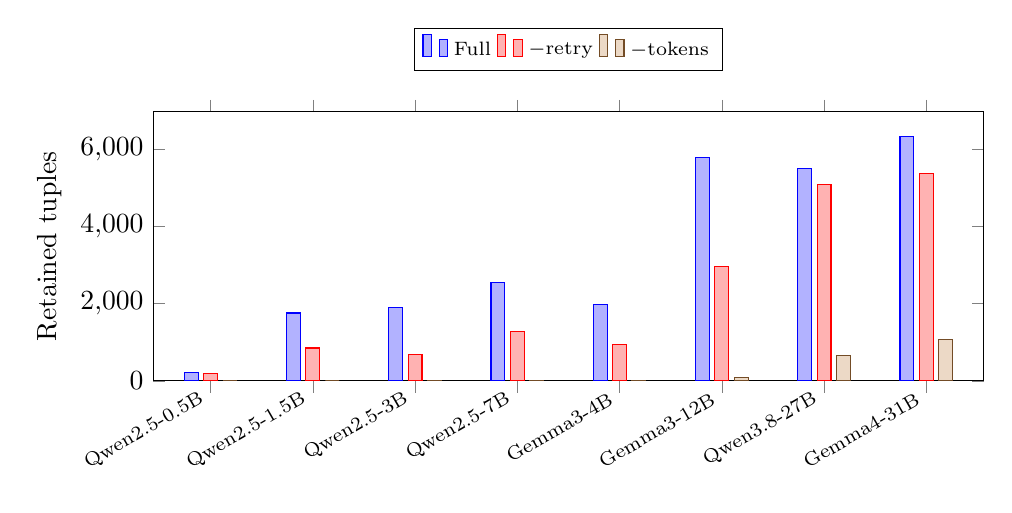
\begin{tikzpicture}
\begin{axis}[
    ybar, bar width=5pt,
    width=\textwidth, height=5cm,
    symbolic x coords={Qwen2.5-0.5B,Qwen2.5-1.5B,Qwen2.5-3B,Qwen2.5-7B,
                        Gemma3-4B,Gemma3-12B,Qwen3.8-27B,Gemma4-31B},
    xtick=data, x tick label style={rotate=30,anchor=east,font=\scriptsize},
    ylabel={Retained tuples}, ymin=0,
    enlarge x limits=0.08,
    legend style={at={(0.5,1.15)}, anchor=south, legend columns=-1, font=\scriptsize},
    nodes near coords style={font=\tiny},
]
\addplot coordinates {
 (Qwen2.5-0.5B,219) (Qwen2.5-1.5B,1760) (Qwen2.5-3B,1909) (Qwen2.5-7B,2546)
 (Gemma3-4B,1969) (Gemma3-12B,5790) (Qwen3.8-27B,5494) (Gemma4-31B,6340)};
\addplot coordinates {
 (Qwen2.5-0.5B,195) (Qwen2.5-1.5B,853) (Qwen2.5-3B,674) (Qwen2.5-7B,1278)
 (Gemma3-4B,938) (Gemma3-12B,2963) (Qwen3.8-27B,5089) (Gemma4-31B,5375)};
\addplot coordinates {
 (Qwen2.5-0.5B,0) (Qwen2.5-1.5B,0) (Qwen2.5-3B,2) (Qwen2.5-7B,7)
 (Gemma3-4B,10) (Gemma3-12B,82) (Qwen3.8-27B,655) (Gemma4-31B,1077)};
\legend{Full, $-$retry, $-$tokens}
\end{axis}
\end{tikzpicture}
\caption{SSA: retained tuples per model and condition.}
\label{fig:ablation-ssa}
\end{subfigure}

\vspace{0.5em}

\begin{subfigure}{\textwidth}
\centering
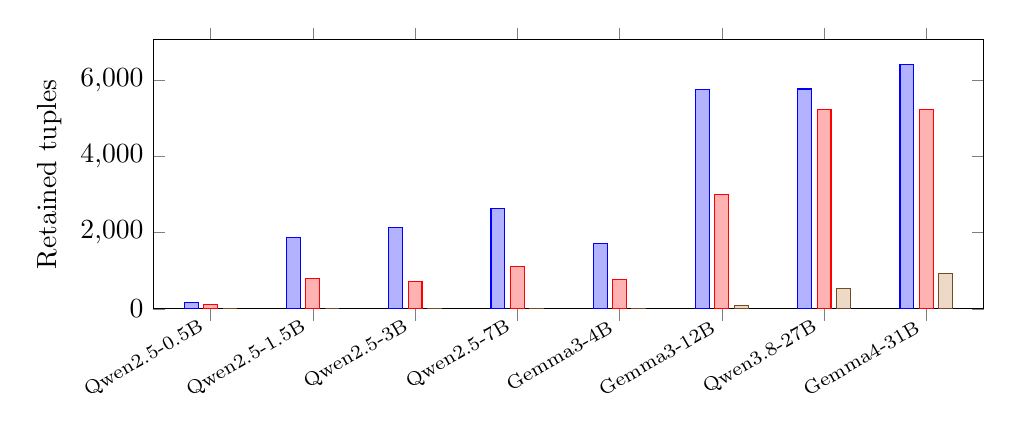
\begin{tikzpicture}
\begin{axis}[
    ybar, bar width=5pt,
    width=\textwidth, height=5cm,
    symbolic x coords={Qwen2.5-0.5B,Qwen2.5-1.5B,Qwen2.5-3B,Qwen2.5-7B,
                        Gemma3-4B,Gemma3-12B,Qwen3.8-27B,Gemma4-31B},
    xtick=data, x tick label style={rotate=30,anchor=east,font=\scriptsize},
    ylabel={Retained tuples}, ymin=0,
    enlarge x limits=0.08,
    nodes near coords style={font=\tiny},
]
\addplot coordinates {
 (Qwen2.5-0.5B,173) (Qwen2.5-1.5B,1869) (Qwen2.5-3B,2132) (Qwen2.5-7B,2642)
 (Gemma3-4B,1707) (Gemma3-12B,5755) (Qwen3.8-27B,5774) (Gemma4-31B,6423)};
\addplot coordinates {
 (Qwen2.5-0.5B,122) (Qwen2.5-1.5B,792) (Qwen2.5-3B,729) (Qwen2.5-7B,1119)
 (Gemma3-4B,766) (Gemma3-12B,3008) (Qwen3.8-27B,5243) (Gemma4-31B,5228)};
\addplot coordinates {
 (Qwen2.5-0.5B,0) (Qwen2.5-1.5B,0) (Qwen2.5-3B,4) (Qwen2.5-7B,8)
 (Gemma3-4B,13) (Gemma3-12B,101) (Qwen3.8-27B,545) (Gemma4-31B,928)};
\end{axis}
\end{tikzpicture}
\caption{ASQP: retained tuples per model and condition.}
\label{fig:ablation-asqp}
\end{subfigure}
\caption{Retained tuples under Full, $-$retry, and $-$tokens conditions, by model and task. Numeric values are in Tables~\ref{tab:reject} and \ref{tab:yield}.}
\label{fig:ablation}
\end{figure*}

\subsection{SSA}
\paragraph{Tokens and retries.}
Gemma 3 12B drops from 5,790 to 2,963 retained tuples without retries. Qwen2.5-7B drops from 2,546 to 1,278. Qwen3.8-27B drops from 5,494 to 5,089 tuples, a smaller proportional loss than the other models. Gemma 4 31B retains 5,375 tuples without retries, compared with 6,340 under Full. This supports corrective feedback as a means of retaining more outputs, without establishing that corrections improve their meaning.

\paragraph{Direct offsets.}
Direct offsets yield fewer annotations in every case, ranging from 0 to 1,077 tuples. Gemma 3 12B retains 82 tuples with direct offsets, versus 5,790 with tokens. Qwen3.8-27B retains 655 tuples with direct offsets, exceeding the smaller models but remaining well below its Full output. Gemma 4 31B retains 1,077 tuples with direct offsets, still substantially fewer than under Full. The comparison supports indexed-token selection for productive, structurally aligned annotation under these prompts.

\subsection{ASQP}
\paragraph{Tokens and retries.}
Gemma 3 12B drops from 5,755 to 3,008 retained tuples without retries. Qwen2.5-7B drops from 2,642 to 1,119. Qwen3.8-27B drops from 5,774 to 5,243 tuples, again a smaller proportional loss than the other models. Gemma 4 31B retains 5,228 tuples without retries, compared with 6,423 under Full. This supports corrective feedback as a means of retaining more outputs, without establishing that corrections improve their meaning.

\paragraph{Direct offsets.}
Direct offsets yield fewer annotations in every case, ranging from 0 to 928 tuples. Qwen2.5-1.5B rejects only 16.4\% of units under direct offsets, yet returns zero annotations and accepts 3,201 empty units. Gemma 3 12B retains 101 tuples with direct offsets, versus 5,755 with tokens. Qwen3.8-27B retains 545 tuples with direct offsets, exceeding the smaller models but remaining well below its Full output. Gemma 4 31B retains 928 tuples with direct offsets, still substantially fewer than under Full. The comparison supports indexed-token selection for productive, structurally aligned annotation under these prompts.

\section{Implications for Annotation Pipelines}
The combined structural and human analyses distinguish three requirements: a span must point to the recorded text, select semantically appropriate words, and connect the appropriate roles. Deterministic mapping and validation address the first requirement. Target substitutions, incomplete expressions, and ambiguous scope remain possible even when every retained interval is aligned.

The reviewed examples also show why more retained tuples need not mean either more errors or better coverage. Some additional outputs identify plausible opinions missing from the supplied reference, while others duplicate an evaluative phrase as its own target. Review should therefore consider the relation in context and preserve reasoned reservations, rather than rewarding reference copying or treating every extra tuple as overannotation.

Boundary design and semantic guidance address different limitations. Finer punctuation-aware indexing could make expressions such as \textit{competente} selectable without the adjoining clause. Clearer scope guidance could help distinguish hotel personnel, other guests, and surrounding entities. These are implications of observed cases, not tested improvements; the experiment keeps tokenization and semantic instructions fixed.

The human evidence remains a purposive, partially reviewed sample with visible model identity and one reviewer. The counts describe inspection coverage and recorded judgments, not population accuracy, inter-annotator agreement, or a model ranking. In particular, reviewing retained tuples cannot establish how many opinions were missed. The contribution of this analysis is to explain concrete successes and failure modes that structural counts alone leave unresolved.

\section{Conclusion}
With task-specific guides, indexed-token selection and corrective retries produce more retained annotations than either ablation for every evaluated model and task. Deterministic offset construction and validation provide source-aligned retained spans. This retention gain comes with lower measured throughput. The partial human audit confirms that source alignment alone does not ensure appropriate opinions, roles, or semantic boundaries.

\section{Limitations}


\bibliography{custom}

\clearpage
\onecolumn

\appendix

\section{Complete Ablations}

\begin{table}[h]
\centering\small
\renewcommand{\arraystretch}{1.08}
\setlength{\tabcolsep}{8pt}
\begin{tabular}{lrrr}
\toprule
\multicolumn{4}{l}{\textbf{SSA}} \\
Model & Full & $-$tokens & $-$retry \\
\midrule
Qwen2.5-0.5B & 94.3 & 99.7 & 94.9 \\
Qwen2.5-1.5B & 67.0 & 97.8 & 83.4 \\
Qwen2.5-3B & 42.1 & 87.6 & 67.0 \\
Qwen2.5-7B & 42.2 & 96.9 & 65.6 \\
Gemma 3 4B & 46.8 & 88.3 & 78.0 \\
Gemma 3 12B & 6.6 & 89.8 & 39.2 \\
Qwen3.8-27B & 0.6 & 72.0 & 5.2 \\
Gemma 4 31B & 1.6 & 71.4 & 12.6 \\
\midrule
\multicolumn{4}{l}{\textbf{ASQP}} \\
Model & Full & $-$tokens & $-$retry \\
\midrule
Qwen2.5-0.5B & 95.6 & 66.9 & 96.9 \\
Qwen2.5-1.5B & 58.2 & 16.4 & 83.1 \\
Qwen2.5-3B & 27.7 & 19.7 & 67.6 \\
Qwen2.5-7B & 34.5 & 86.5 & 65.8 \\
Gemma 3 4B & 58.9 & 89.7 & 82.8 \\
Gemma 3 12B & 4.6 & 86.8 & 37.8 \\
Qwen3.8-27B & 0.4 & 70.8 & 4.3 \\
Gemma 4 31B & 0.4 & 69.0 & 11.8 \\
\bottomrule
\end{tabular}
\caption{Rejection rates (\%). All conditions use the same sentence segmentation and validation. $-$tokens generates character positions directly; $-$retry disables corrective attempts.}
\label{tab:reject}
\end{table}
\begin{table}[!ht]
\centering\small
\renewcommand{\arraystretch}{1.08}
\setlength{\tabcolsep}{8pt}
\begin{tabular}{lrrr}
\toprule
\multicolumn{4}{l}{\textbf{SSA}} \\
Model & Full & $-$tokens & $-$retry \\
\midrule
Qwen2.5-0.5B & 219 & 0 & 195 \\
Qwen2.5-1.5B & 1,760 & 0 & 853 \\
Qwen2.5-3B & 1,909 & 2 & 674 \\
Qwen2.5-7B & 2,546 & 7 & 1,278 \\
Gemma 3 4B & 1,969 & 10 & 938 \\
Gemma 3 12B & 5,790 & 82 & 2,963 \\
Qwen3.8-27B & 5,494 & 655 & 5,089 \\
Gemma 4 31B & 6,340 & 1,077 & 5,375 \\
\midrule
\multicolumn{4}{l}{\textbf{ASQP}} \\
Model & Full & $-$tokens & $-$retry \\
\midrule
Qwen2.5-0.5B & 173 & 0 & 122 \\
Qwen2.5-1.5B & 1,869 & 0 & 792 \\
Qwen2.5-3B & 2,132 & 4 & 729 \\
Qwen2.5-7B & 2,642 & 8 & 1,119 \\
Gemma 3 4B & 1,707 & 13 & 766 \\
Gemma 3 12B & 5,755 & 101 & 3,008 \\
Qwen3.8-27B & 5,774 & 545 & 5,243 \\
Gemma 4 31B & 6,423 & 928 & 5,228 \\
\bottomrule
\end{tabular}
\caption{Retained annotation counts. Output quantity does not establish semantic quality or coverage.}
\label{tab:yield}
\end{table}
\clearpage
\twocolumn

\section{Qualitative Annotation Analysis}
\label{app:qualitative}
We inspect one retained Full SSA annotation and one retained Full ASQP annotation for each Qwen2.5 and Gemma 3 model, selected purposively from short sentences to illustrate interpretable outputs and limitations. Qwen3.8-27B is examined through the human-reviewed cases in Section~\ref{app:human}. These twelve cases are not a representative sample or independent human adjudication. Each entry shows one tuple, not all annotations for the sentence. Source IDs and document-level half-open offsets are retained for verification; all displayed spans were checked against the source text.

\subsection{Qwen2.5-0.5B}

\paragraph{SSA (\texttt{ex\_0403}).}
\textit{``Hotel com condições gerais muito más.''} Aspect: \textit{condições} $[10,19)$; opinion: \textit{muito} $[27,32)$; polarity: POS. Holder: \textit{Hotel} $[0,5)$. The hotel is incorrectly assigned as opinion holder. Positive polarity contradicts the complaint, and the intensifier alone omits the negative adjective.

\paragraph{ASQP (\texttt{ex\_0931}).}
\textit{``A localização central é ótima.''} Aspect: \textit{localização} $[57,68)$; opinion: \textit{ótima.} $[79,85)$; polarity: POS. Category: location. Location, positive polarity, and the evaluative adjective form a coherent annotation. Attached sentence punctuation remains in the selected opinion token.

\subsection{Qwen2.5-1.5B}

\paragraph{SSA (\texttt{ex\_0403}).}
\textit{``Quarto sem tv e com pouca privacidade, uma vez que a cortina era transparente.''} Aspect: \textit{Quarto} $[282,288)$; opinion: \textit{sem tv e com pouca privacidade, uma vez que a cortina era transparente.} $[289,360)$; polarity: NEG. Holder: null. The room and negative polarity capture the complaint, but the opinion span includes the entire causal explanation and is broader than necessary.

\paragraph{ASQP (\texttt{ex\_0403}).}
\textit{``Para as condições que tem é demasiado caro.''} Aspect: \textit{condições que} $[612,625)$; opinion: \textit{demasiado} $[632,641)$; polarity: NEG. Category: price. The price category fits the complaint, but the aspect includes a trailing relative word and the opinion omits the evaluative adjective meaning expensive.

\subsection{Qwen2.5-3B}

\paragraph{SSA (\texttt{ex\_0403}).}
\textit{``Hotel com condições gerais muito más.''} Aspect: \textit{condições gerais muito} $[10,32)$; opinion: \textit{más.} $[33,37)$; polarity: NEG. Holder: \textit{Hotel} $[0,5)$. Negative polarity fits, but the hotel is not the opinion holder; the aspect also absorbs an intensifier belonging to the evaluation.

\paragraph{ASQP (\texttt{ex\_1024}).}
\textit{``Os quartos são pequenos e quase não tem espaço para as malas.''} Aspect: \textit{quartos} $[243,250)$; opinion: \textit{pequenos} $[255,263)$; polarity: NEG. Category: structure. The room target and its small size support a coherent negative structural evaluation. The selection isolates an interpretable target--opinion pair.

\subsection{Qwen2.5-7B}

\paragraph{SSA (\texttt{ex\_0403}).}
\textit{``Hotel com condições gerais muito más.''} Aspect: \textit{condições gerais} $[10,26)$; opinion: \textit{muito más.} $[27,37)$; polarity: NEG. Holder: null. The null holder and complete negative expression fit a direct complaint about general conditions. The spans preserve the evaluative intensifier.

\paragraph{ASQP (\texttt{ex\_1024}).}
\textit{``O hotel segue corretamente os padrões do Mercure o que significa ser bom.''} Aspect: \textit{hotel} $[2,7)$; opinion: \textit{bom.} $[69,73)$; polarity: POS. Category: general. The hotel and positive adjective form a plausible pair, but the sentiment is marked implicit despite an overt evaluative word.

\subsection{Gemma 3 4B}

\paragraph{SSA (\texttt{ex\_0403}).}
\textit{``Hotel com condições gerais muito más.''} Aspect: \textit{condições gerais} $[10,26)$; opinion: \textit{muito más.} $[27,37)$; polarity: NEG. Holder: null. The model retains a plausible target and complete negative expression with a null holder. This shows an interpretable output among the retained annotations.

\paragraph{ASQP (\texttt{ex\_1024}).}
\textit{``A funcionária que me recebeu na recepção visivelmente não gosta de brasileiros o que causou uma impressão ruim.''} Aspect: \textit{funcionária} $[130,141)$; opinion: \textit{gosta} $[186,191)$; polarity: NEG. Category: service. The service category and negative polarity fit the complaint, but the selected verb omits its preceding negation. Correct offsets do not preserve the intended meaning of an incomplete expression.

\subsection{Gemma 3 12B}

\paragraph{SSA (\texttt{ex\_0403}).}
\textit{``isolamento acústico muito fraco, pelo que se ouvia no piso todo sempre que alguém passava no corredor.''} Aspect: \textit{isolamento acústico} $[361,380)$; opinion: \textit{muito fraco,} $[381,393)$; polarity: NEG. Holder: null. The acoustic-insulation target and full negative expression are coherent, with no unsupported holder attribution.

\paragraph{ASQP (\texttt{ex\_0403}).}
\textit{``Hotel com condições gerais muito más.''} Aspect: \textit{Hotel} $[0,5)$; opinion: \textit{muito más.} $[27,37)$; polarity: NEG. Category: general. The general category, hotel target, and complete negative expression provide a coherent reading of the complaint.

\onecolumn
\section{Operational Analysis}
\label{app:operations}
Attempts and retained tuples are counted from the records; time is the final JSON's runner wall time, excluding download and server startup. With 200 concurrent units, it is not individual request latency. Automatic client transport retries may not be included in application-level counts. No token usage, energy, monetary cost, or repeated timing trials are available. Cumulative retry metadata cannot establish the outcome of a counterfactual one-retry run.
\begin{table}[!ht]
\centering\small
\begin{tabular}{lrrrrr}
\toprule
Model & Attempts/unit & \multicolumn{2}{c}{Minutes} & \multicolumn{2}{c}{Tuples/minute}\\
 & Full & Full & $-$retry & Full & $-$retry\\
\midrule
\multicolumn{6}{l}{\textbf{SSA}} \\
Qwen2.5-0.5B & 3.83 & 3.00 & 0.68 & 72.9 & 285.7 \\
Qwen2.5-1.5B & 3.23 & 5.04 & 1.11 & 349.0 & 770.1 \\
Qwen2.5-3B & 2.66 & 8.77 & 2.20 & 217.6 & 305.9 \\
Qwen2.5-7B & 2.58 & 14.68 & 4.08 & 173.5 & 313.5 \\
Gemma 3 4B & 2.97 & 5.74 & 1.78 & 343.0 & 527.1 \\
Gemma 3 12B & 1.56 & 11.25 & 4.68 & 514.7 & 633.4 \\
Qwen3.8-27B & 1.07 & 15.57 & 13.29 & 352.8 & 383.0 \\
Gemma 4 31B & 1.19 & 42.18 & 28.38 & 150.3 & 189.4 \\
\midrule
\multicolumn{6}{l}{\textbf{ASQP}} \\
Qwen2.5-0.5B & 3.88 & 3.35 & 0.88 & 51.7 & 138.4 \\
Qwen2.5-1.5B & 3.08 & 4.57 & 1.26 & 409.1 & 630.7 \\
Qwen2.5-3B & 2.49 & 7.54 & 2.19 & 282.9 & 333.1 \\
Qwen2.5-7B & 2.44 & 14.15 & 4.35 & 186.8 & 257.2 \\
Gemma 3 4B & 3.14 & 4.82 & 1.53 & 353.8 & 502.2 \\
Gemma 3 12B & 1.50 & 10.04 & 4.39 & 573.1 & 684.8 \\
Qwen3.8-27B & 1.05 & 17.03 & 13.98 & 339.1 & 375.0 \\
Gemma 4 31B & 1.13 & 36.95 & 26.00 & 173.8 & 201.1 \\
\bottomrule
\end{tabular}
\caption{Operational comparison on 763 documents and 3,831 units per row. No-retry makes one application-level attempt per unit. Output rates measure quantity, not semantic quality.}
\label{tab:ops}
\end{table}

% Generated by scripts/semantic_audit_report.py from the semantic audit (audit/GUIA_AUDITORIA_SEMANTICA.md). Do not edit by hand.
\section{Semantic Audit of Retained Annotations}
\label{app:semantic_audit}
Structural validation guarantees that every retained span matches its source substring, not that the tuple is meaningful. We therefore estimate, for each model, the share of retained tuples that a hotel manager would accept as a guest opinion about the hotel or the stay. For each of the 44 runs with retained tuples we draw up to 50 tuples uniformly without replacement (seed 20260930); runs with fewer tuples are judged completely. This yields 1,944 sampled tuples and 1,817 unique items, since identical tuples in different runs are judged once. Each tuple is judged in the context of its sentence and the neighboring sentences, following a written guide with error codes for the aspect, opinion expression, category (ASQP), polarity and holder (SSA).

A tuple is \emph{invalid} when it contains no evaluation, when its aspect is not a target (a function word, an evaluative word or a whole clause), when its aspect is a named place or landmark (a street name, a monument, a city), when its aspect is another out-of-domain entity (another establishment, the guest, the weather, a booking platform), or when its expression is not evaluative. It is \emph{partial} when it records an in-domain opinion but has a wrong category, polarity or holder, a mispaired aspect, or an incomplete or excessive expression; otherwise it is \emph{valid}. Generic surroundings that describe the hotel's location, such as proximity to the metro or a safe neighborhood, count as in-domain location opinions.

The judgments were produced by LLM judges (Claude Opus 5.5) following the guide, not by human annotators. 184 items were judged twice without the judges' knowledge: raw agreement on the three-way verdict is 93.5\% (Cohen's $\kappa=0.89$). Because both judges are the same model, this measures consistency rather than validity. A second pass re-examined the 141 out-of-domain codes under the location rule above and reclassified 57 of them as accepted surroundings. The rates should be checked against a human-reviewed subsample before they are read as human evaluation.

Across all 90,306 retained tuples, an estimated 66.8\% are valid and 82.0\% record an in-domain opinion. Named places or landmarks as aspects account for 2.2\%, other out-of-domain entities for 3.3\%, and tuples without an opinion for 6.5\%.

Tables~\ref{tab:audit-qwen25-05b}--\ref{tab:audit-gemma431b} report one table per model. \emph{Strict} is the share of valid tuples; \emph{Domain} adds partial tuples; \emph{Named place} and \emph{Other entity} are the two out-of-domain codes; \emph{No opinion} covers tuples without an evaluation or with a non-evaluative expression. Rates are percentages of retained tuples; brackets give 95\% Wilson intervals; $^\dagger$ marks runs judged completely. \emph{Est.\ valid} multiplies the strict rate by the retained tuples. Totals weight each run by its retained tuples. With 50 judged tuples, a run's interval spans roughly $\pm$13 points, so differences between conditions of the same model are often within the margin.

\begin{table}[!ht]
\centering\footnotesize
\setlength{\tabcolsep}{4pt}
\begin{tabular}{lrrrrrrrr}
\toprule
Condition & Retained & Judged & Est.\ valid & Strict & Domain & Named place & Other entity & No opinion \\
\midrule
\multicolumn{9}{l}{\textbf{SSA}} \\
Full & 219 & 50 & 48 & 22.0 {\scriptsize[13--35]} & 68.0 {\scriptsize[54--79]} & 2.0 {\scriptsize[0--10]} & 2.0 {\scriptsize[0--10]} & 16.0 {\scriptsize[8--29]} \\
$-$tokens & 0 & 0 & 0 & -- & -- & -- & -- & -- \\
$-$retry & 195 & 50 & 27 & 14.0 {\scriptsize[7--26]} & 62.0 {\scriptsize[48--74]} & 2.0 {\scriptsize[0--10]} & 4.0 {\scriptsize[1--13]} & 28.0 {\scriptsize[17--42]} \\
\midrule
\multicolumn{9}{l}{\textbf{ASQP}} \\
Full & 173 & 50 & 48 & 28.0 {\scriptsize[17--42]} & 62.0 {\scriptsize[48--74]} & 0.0 {\scriptsize[0--7]} & 0.0 {\scriptsize[0--7]} & 24.0 {\scriptsize[14--37]} \\
$-$tokens & 0 & 0 & 0 & -- & -- & -- & -- & -- \\
$-$retry & 122 & 50 & 41 & 34.0 {\scriptsize[22--48]} & 66.0 {\scriptsize[52--78]} & 0.0 {\scriptsize[0--7]} & 4.0 {\scriptsize[1--13]} & 14.0 {\scriptsize[7--26]} \\
\midrule
Total & 709 & 200 & 164 & 23.3 {\scriptsize[18--28]} & 64.5 {\scriptsize[59--70]} & 1.2 {\scriptsize[0--3]} & 2.4 {\scriptsize[1--4]} & 20.9 {\scriptsize[16--26]} \\
\bottomrule
\end{tabular}
\caption{Semantic audit of Qwen2.5-0.5B: estimated validity of retained tuples (\%) by task and condition.}
\label{tab:audit-qwen25-05b}
\end{table}

\begin{table}[!ht]
\centering\footnotesize
\setlength{\tabcolsep}{4pt}
\begin{tabular}{lrrrrrrrr}
\toprule
Condition & Retained & Judged & Est.\ valid & Strict & Domain & Named place & Other entity & No opinion \\
\midrule
\multicolumn{9}{l}{\textbf{SSA}} \\
Full & 1,760 & 50 & 387 & 22.0 {\scriptsize[13--35]} & 62.0 {\scriptsize[48--74]} & 0.0 {\scriptsize[0--7]} & 2.0 {\scriptsize[0--10]} & 28.0 {\scriptsize[17--42]} \\
$-$tokens & 0 & 0 & 0 & -- & -- & -- & -- & -- \\
$-$retry & 853 & 50 & 290 & 34.0 {\scriptsize[22--48]} & 58.0 {\scriptsize[44--71]} & 6.0 {\scriptsize[2--16]} & 4.0 {\scriptsize[1--13]} & 26.0 {\scriptsize[16--40]} \\
\midrule
\multicolumn{9}{l}{\textbf{ASQP}} \\
Full & 1,869 & 50 & 598 & 32.0 {\scriptsize[21--46]} & 50.0 {\scriptsize[37--63]} & 2.0 {\scriptsize[0--10]} & 12.0 {\scriptsize[6--24]} & 34.0 {\scriptsize[22--48]} \\
$-$tokens & 0 & 0 & 0 & -- & -- & -- & -- & -- \\
$-$retry & 792 & 50 & 253 & 32.0 {\scriptsize[21--46]} & 52.0 {\scriptsize[39--65]} & 4.0 {\scriptsize[1--13]} & 2.0 {\scriptsize[0--10]} & 30.0 {\scriptsize[19--44]} \\
\midrule
Total & 5,274 & 200 & 1,528 & 29.0 {\scriptsize[22--36]} & 55.6 {\scriptsize[48--63]} & 2.3 {\scriptsize[0--4]} & 5.9 {\scriptsize[2--9]} & 30.1 {\scriptsize[23--37]} \\
\bottomrule
\end{tabular}
\caption{Semantic audit of Qwen2.5-1.5B: estimated validity of retained tuples (\%) by task and condition.}
\label{tab:audit-qwen25-15b}
\end{table}

\begin{table}[!ht]
\centering\footnotesize
\setlength{\tabcolsep}{4pt}
\begin{tabular}{lrrrrrrrr}
\toprule
Condition & Retained & Judged & Est.\ valid & Strict & Domain & Named place & Other entity & No opinion \\
\midrule
\multicolumn{9}{l}{\textbf{SSA}} \\
Full & 1,909 & 50 & 229 & 12.0 {\scriptsize[6--24]} & 70.0 {\scriptsize[56--81]} & 4.0 {\scriptsize[1--13]} & 0.0 {\scriptsize[0--7]} & 16.0 {\scriptsize[8--29]} \\
$-$tokens & 2 & 2 & 2 & 100.0$^\dagger$ & 100.0$^\dagger$ & 0.0$^\dagger$ & 0.0$^\dagger$ & 0.0$^\dagger$ \\
$-$retry & 674 & 50 & 148 & 22.0 {\scriptsize[13--35]} & 74.0 {\scriptsize[60--84]} & 2.0 {\scriptsize[0--10]} & 6.0 {\scriptsize[2--16]} & 10.0 {\scriptsize[4--21]} \\
\midrule
\multicolumn{9}{l}{\textbf{ASQP}} \\
Full & 2,132 & 50 & 768 & 36.0 {\scriptsize[24--50]} & 54.0 {\scriptsize[40--67]} & 2.0 {\scriptsize[0--10]} & 0.0 {\scriptsize[0--7]} & 32.0 {\scriptsize[21--46]} \\
$-$tokens & 4 & 4 & 3 & 75.0$^\dagger$ & 75.0$^\dagger$ & 0.0$^\dagger$ & 0.0$^\dagger$ & 0.0$^\dagger$ \\
$-$retry & 729 & 50 & 554 & 76.0 {\scriptsize[63--86]} & 86.0 {\scriptsize[74--93]} & 0.0 {\scriptsize[0--7]} & 0.0 {\scriptsize[0--7]} & 4.0 {\scriptsize[1--13]} \\
\midrule
Total & 5,450 & 206 & 1,704 & 31.3 {\scriptsize[25--38]} & 66.4 {\scriptsize[59--74]} & 2.4 {\scriptsize[0--5]} & 0.7 {\scriptsize[0--2]} & 19.9 {\scriptsize[14--26]} \\
\bottomrule
\end{tabular}
\caption{Semantic audit of Qwen2.5-3B: estimated validity of retained tuples (\%) by task and condition.}
\label{tab:audit-qwen25-3b}
\end{table}

\begin{table}[!ht]
\centering\footnotesize
\setlength{\tabcolsep}{4pt}
\begin{tabular}{lrrrrrrrr}
\toprule
Condition & Retained & Judged & Est.\ valid & Strict & Domain & Named place & Other entity & No opinion \\
\midrule
\multicolumn{9}{l}{\textbf{SSA}} \\
Full & 2,546 & 50 & 1,069 & 42.0 {\scriptsize[29--56]} & 74.0 {\scriptsize[60--84]} & 2.0 {\scriptsize[0--10]} & 2.0 {\scriptsize[0--10]} & 18.0 {\scriptsize[10--31]} \\
$-$tokens & 7 & 7 & 5 & 71.4$^\dagger$ & 71.4$^\dagger$ & 0.0$^\dagger$ & 0.0$^\dagger$ & 0.0$^\dagger$ \\
$-$retry & 1,278 & 50 & 869 & 68.0 {\scriptsize[54--79]} & 92.0 {\scriptsize[81--97]} & 0.0 {\scriptsize[0--7]} & 0.0 {\scriptsize[0--7]} & 4.0 {\scriptsize[1--13]} \\
\midrule
\multicolumn{9}{l}{\textbf{ASQP}} \\
Full & 2,642 & 50 & 1,427 & 54.0 {\scriptsize[40--67]} & 78.0 {\scriptsize[65--87]} & 2.0 {\scriptsize[0--10]} & 0.0 {\scriptsize[0--7]} & 6.0 {\scriptsize[2--16]} \\
$-$tokens & 8 & 8 & 7 & 87.5$^\dagger$ & 100.0$^\dagger$ & 0.0$^\dagger$ & 0.0$^\dagger$ & 0.0$^\dagger$ \\
$-$retry & 1,119 & 50 & 895 & 80.0 {\scriptsize[67--89]} & 86.0 {\scriptsize[74--93]} & 2.0 {\scriptsize[0--10]} & 6.0 {\scriptsize[2--16]} & 2.0 {\scriptsize[0--10]} \\
\midrule
Total & 7,600 & 215 & 4,272 & 56.2 {\scriptsize[49--63]} & 80.2 {\scriptsize[74--86]} & 1.7 {\scriptsize[0--4]} & 1.6 {\scriptsize[0--3]} & 9.1 {\scriptsize[5--13]} \\
\bottomrule
\end{tabular}
\caption{Semantic audit of Qwen2.5-7B: estimated validity of retained tuples (\%) by task and condition.}
\label{tab:audit-qwen25-7b}
\end{table}

\begin{table}[!ht]
\centering\footnotesize
\setlength{\tabcolsep}{4pt}
\begin{tabular}{lrrrrrrrr}
\toprule
Condition & Retained & Judged & Est.\ valid & Strict & Domain & Named place & Other entity & No opinion \\
\midrule
\multicolumn{9}{l}{\textbf{SSA}} \\
Full & 1,969 & 50 & 1,300 & 66.0 {\scriptsize[52--78]} & 82.0 {\scriptsize[69--90]} & 2.0 {\scriptsize[0--10]} & 4.0 {\scriptsize[1--13]} & 2.0 {\scriptsize[0--10]} \\
$-$tokens & 10 & 10 & 7 & 70.0$^\dagger$ & 90.0$^\dagger$ & 0.0$^\dagger$ & 0.0$^\dagger$ & 0.0$^\dagger$ \\
$-$retry & 938 & 50 & 638 & 68.0 {\scriptsize[54--79]} & 80.0 {\scriptsize[67--89]} & 0.0 {\scriptsize[0--7]} & 2.0 {\scriptsize[0--10]} & 14.0 {\scriptsize[7--26]} \\
\midrule
\multicolumn{9}{l}{\textbf{ASQP}} \\
Full & 1,707 & 50 & 751 & 44.0 {\scriptsize[31--58]} & 70.0 {\scriptsize[56--81]} & 0.0 {\scriptsize[0--7]} & 0.0 {\scriptsize[0--7]} & 12.0 {\scriptsize[6--24]} \\
$-$tokens & 13 & 13 & 4 & 30.8$^\dagger$ & 53.8$^\dagger$ & 7.7$^\dagger$ & 0.0$^\dagger$ & 15.4$^\dagger$ \\
$-$retry & 766 & 50 & 398 & 52.0 {\scriptsize[39--65]} & 76.0 {\scriptsize[63--86]} & 2.0 {\scriptsize[0--10]} & 2.0 {\scriptsize[0--10]} & 18.0 {\scriptsize[10--31]} \\
\midrule
Total & 5,403 & 223 & 3,098 & 57.3 {\scriptsize[50--64]} & 77.0 {\scriptsize[71--83]} & 1.0 {\scriptsize[0--3]} & 2.1 {\scriptsize[0--4]} & 9.5 {\scriptsize[6--13]} \\
\bottomrule
\end{tabular}
\caption{Semantic audit of Gemma 3 4B: estimated validity of retained tuples (\%) by task and condition.}
\label{tab:audit-gemma34b}
\end{table}

\begin{table}[!ht]
\centering\footnotesize
\setlength{\tabcolsep}{4pt}
\begin{tabular}{lrrrrrrrr}
\toprule
Condition & Retained & Judged & Est.\ valid & Strict & Domain & Named place & Other entity & No opinion \\
\midrule
\multicolumn{9}{l}{\textbf{SSA}} \\
Full & 5,790 & 50 & 4,053 & 70.0 {\scriptsize[56--81]} & 82.0 {\scriptsize[69--90]} & 8.0 {\scriptsize[3--19]} & 4.0 {\scriptsize[1--13]} & 2.0 {\scriptsize[0--10]} \\
$-$tokens & 82 & 50 & 52 & 64.0 {\scriptsize[50--76]} & 72.0 {\scriptsize[58--83]} & 0.0 {\scriptsize[0--7]} & 0.0 {\scriptsize[0--7]} & 6.0 {\scriptsize[2--16]} \\
$-$retry & 2,963 & 50 & 2,015 & 68.0 {\scriptsize[54--79]} & 80.0 {\scriptsize[67--89]} & 2.0 {\scriptsize[0--10]} & 4.0 {\scriptsize[1--13]} & 12.0 {\scriptsize[6--24]} \\
\midrule
\multicolumn{9}{l}{\textbf{ASQP}} \\
Full & 5,755 & 50 & 3,568 & 62.0 {\scriptsize[48--74]} & 72.0 {\scriptsize[58--83]} & 2.0 {\scriptsize[0--10]} & 4.0 {\scriptsize[1--13]} & 10.0 {\scriptsize[4--21]} \\
$-$tokens & 101 & 50 & 44 & 44.0 {\scriptsize[31--58]} & 58.0 {\scriptsize[44--71]} & 0.0 {\scriptsize[0--7]} & 4.0 {\scriptsize[1--13]} & 4.0 {\scriptsize[1--13]} \\
$-$retry & 3,008 & 50 & 1,805 & 60.0 {\scriptsize[46--72]} & 82.0 {\scriptsize[69--90]} & 2.0 {\scriptsize[0--10]} & 2.0 {\scriptsize[0--10]} & 8.0 {\scriptsize[3--19]} \\
\midrule
Total & 17,699 & 300 & 11,537 & 65.2 {\scriptsize[58--72]} & 78.2 {\scriptsize[72--84]} & 3.9 {\scriptsize[1--7]} & 3.6 {\scriptsize[1--6]} & 7.3 {\scriptsize[4--11]} \\
\bottomrule
\end{tabular}
\caption{Semantic audit of Gemma 3 12B: estimated validity of retained tuples (\%) by task and condition.}
\label{tab:audit-gemma312b}
\end{table}

\begin{table}[!ht]
\centering\footnotesize
\setlength{\tabcolsep}{4pt}
\begin{tabular}{lrrrrrrrr}
\toprule
Condition & Retained & Judged & Est.\ valid & Strict & Domain & Named place & Other entity & No opinion \\
\midrule
\multicolumn{9}{l}{\textbf{SSA}} \\
Full & 5,494 & 50 & 4,725 & 86.0 {\scriptsize[74--93]} & 92.0 {\scriptsize[81--97]} & 2.0 {\scriptsize[0--10]} & 4.0 {\scriptsize[1--13]} & 4.0 {\scriptsize[1--13]} \\
$-$tokens & 655 & 50 & 432 & 66.0 {\scriptsize[52--78]} & 76.0 {\scriptsize[63--86]} & 2.0 {\scriptsize[0--10]} & 0.0 {\scriptsize[0--7]} & 0.0 {\scriptsize[0--7]} \\
$-$retry & 5,089 & 50 & 4,377 & 86.0 {\scriptsize[74--93]} & 92.0 {\scriptsize[81--97]} & 0.0 {\scriptsize[0--7]} & 2.0 {\scriptsize[0--10]} & 0.0 {\scriptsize[0--7]} \\
\midrule
\multicolumn{9}{l}{\textbf{ASQP}} \\
Full & 5,774 & 50 & 4,504 & 78.0 {\scriptsize[65--87]} & 88.0 {\scriptsize[76--94]} & 6.0 {\scriptsize[2--16]} & 4.0 {\scriptsize[1--13]} & 2.0 {\scriptsize[0--10]} \\
$-$tokens & 545 & 50 & 338 & 62.0 {\scriptsize[48--74]} & 74.0 {\scriptsize[60--84]} & 0.0 {\scriptsize[0--7]} & 0.0 {\scriptsize[0--7]} & 0.0 {\scriptsize[0--7]} \\
$-$retry & 5,243 & 50 & 4,299 & 82.0 {\scriptsize[69--90]} & 90.0 {\scriptsize[79--96]} & 4.0 {\scriptsize[1--13]} & 6.0 {\scriptsize[2--16]} & 0.0 {\scriptsize[0--7]} \\
\midrule
Total & 22,800 & 300 & 18,675 & 81.9 {\scriptsize[77--87]} & 89.6 {\scriptsize[86--94]} & 3.0 {\scriptsize[1--5]} & 3.8 {\scriptsize[1--6]} & 1.5 {\scriptsize[0--3]} \\
\bottomrule
\end{tabular}
\caption{Semantic audit of Qwen3.8-27B: estimated validity of retained tuples (\%) by task and condition.}
\label{tab:audit-qwen38-27b}
\end{table}

\begin{table}[!ht]
\centering\footnotesize
\setlength{\tabcolsep}{4pt}
\begin{tabular}{lrrrrrrrr}
\toprule
Condition & Retained & Judged & Est.\ valid & Strict & Domain & Named place & Other entity & No opinion \\
\midrule
\multicolumn{9}{l}{\textbf{SSA}} \\
Full & 6,340 & 50 & 4,311 & 68.0 {\scriptsize[54--79]} & 84.0 {\scriptsize[71--92]} & 0.0 {\scriptsize[0--7]} & 10.0 {\scriptsize[4--21]} & 0.0 {\scriptsize[0--7]} \\
$-$tokens & 1,077 & 50 & 775 & 72.0 {\scriptsize[58--83]} & 80.0 {\scriptsize[67--89]} & 2.0 {\scriptsize[0--10]} & 4.0 {\scriptsize[1--13]} & 2.0 {\scriptsize[0--10]} \\
$-$retry & 5,375 & 50 & 3,655 & 68.0 {\scriptsize[54--79]} & 86.0 {\scriptsize[74--93]} & 2.0 {\scriptsize[0--10]} & 4.0 {\scriptsize[1--13]} & 0.0 {\scriptsize[0--7]} \\
\midrule
\multicolumn{9}{l}{\textbf{ASQP}} \\
Full & 6,423 & 50 & 5,652 & 88.0 {\scriptsize[76--94]} & 94.0 {\scriptsize[84--98]} & 0.0 {\scriptsize[0--7]} & 0.0 {\scriptsize[0--7]} & 2.0 {\scriptsize[0--10]} \\
$-$tokens & 928 & 50 & 687 & 74.0 {\scriptsize[60--84]} & 76.0 {\scriptsize[63--86]} & 2.0 {\scriptsize[0--10]} & 0.0 {\scriptsize[0--7]} & 4.0 {\scriptsize[1--13]} \\
$-$retry & 5,228 & 50 & 4,287 & 82.0 {\scriptsize[69--90]} & 94.0 {\scriptsize[84--98]} & 0.0 {\scriptsize[0--7]} & 0.0 {\scriptsize[0--7]} & 0.0 {\scriptsize[0--7]} \\
\midrule
Total & 25,371 & 300 & 19,367 & 76.3 {\scriptsize[71--82]} & 88.6 {\scriptsize[85--92]} & 0.6 {\scriptsize[0--1]} & 3.5 {\scriptsize[1--6]} & 0.7 {\scriptsize[0--2]} \\
\bottomrule
\end{tabular}
\caption{Semantic audit of Gemma 4 31B: estimated validity of retained tuples (\%) by task and condition.}
\label{tab:audit-gemma431b}
\end{table}
\clearpage

\section{Prompt Templates and Annotation Guides}
\label{app:prompts}
These blocks reproduce the model-facing instructions in Portuguese, with
editorial line wrapping. Each system message combines representation-specific
instructions and the task guide. Full and $-$retry share the token prompt.
Direct offsets use the direct instructions and the guide with every occurrence
of \texttt{token\_ids} replaced by \texttt{location}. Complete direct messages
were checked for absence of token-ID cues. The full Hontology file is not sent
to the model.

\subsection{Token-selection system instructions}

\paragraph{SSA}\mbox{}\par
\begin{promptbox}
Você é especialista em análise de sentimento estruturada em português. Você
receberá uma frase e TAGS de tokens indexados. Extraia TODAS as opiniões.
Responda somente um objeto JSON \{"annotations": [...]\}. Use apenas
token\_ids existentes, únicos, crescentes e contíguos. O campo term deve ser
exatamente o trecho formado do primeiro ao último token, incluindo pontuação
quando ela faz parte do token. Use o menor span semanticamente suficiente.
Nunca invente texto. aspect e sentiment devem ter ao menos um token. polarity
deve ser POS, NEG ou NEU. sentiment.type deve ser explicit ou implicit; use
explicit sempre que houver expressão avaliativa textual. Se não houver opinião,
retorne \{"annotations": []\}.

Cada anotação tem holder, aspect, sentiment e polarity. Holder é quem expressa
a opinião; se não estiver expresso, use
\{"term":"null","token\_ids":[]\}. Formato:
\{"holder":\{"term":str,"token\_ids":[int]\},
"aspect":\{"term":str,"token\_ids":[int]\},
"sentiment":\{"term":str,"token\_ids":[int],"type":"explicit"\},
"polarity":"POS"\}. Não confunda sujeito sintático com holder: holder precisa
ser o emissor da avaliação.
\end{promptbox}

\paragraph{ASQP}\mbox{}\par
\begin{promptbox}
Você é especialista em análise de sentimento estruturada em português. Você
receberá uma frase e TAGS de tokens indexados. Extraia TODAS as opiniões.
Responda somente um objeto JSON \{"annotations": [...]\}. Use apenas
token\_ids existentes, únicos, crescentes e contíguos. O campo term deve ser
exatamente o trecho formado do primeiro ao último token, incluindo pontuação
quando ela faz parte do token. Use o menor span semanticamente suficiente.
Nunca invente texto. aspect e sentiment devem ter ao menos um token. polarity
deve ser POS, NEG ou NEU. sentiment.type deve ser explicit ou implicit; use
explicit sempre que houver expressão avaliativa textual. Se não houver opinião,
retorne \{"annotations": []\}.

Cada anotação tem category, aspect, sentiment e polarity. category deve ser
exatamente uma de: structure, service, location, general, price, others.
Formato: \{"category":"structure", "aspect":\{"term":str,"token\_ids":[int]\},
"sentiment":\{"term":str,"token\_ids":[int],"type":"explicit"\},
"polarity":"POS"\}.
\end{promptbox}

\subsection{Direct-offset system instructions}

\paragraph{SSA}\mbox{}\par
\begin{promptbox}
Voce e especialista em analise de sentimento estruturada em portugues. Extraia
TODAS as opinioes e responda somente JSON \{"annotations":[...]\}. Cada span usa
location=[inicio,fim], caracteres relativos ao TEXTO, com inicio inclusivo e fim
exclusivo; term deve ser exatamente TEXTO[inicio:fim]. Use o menor span
suficiente. polarity: POS, NEG ou NEU. sentiment.type: explicit ou implicit.
Campos: holder, aspect, sentiment, polarity. Holder e o emissor; se ausente use
\{"term":"null","location":[]\}. Aspect e sentiment nunca sao vazios.
\end{promptbox}

\paragraph{ASQP}\mbox{}\par
\begin{promptbox}
Voce e especialista em analise de sentimento estruturada em portugues. Extraia
TODAS as opinioes e responda somente JSON \{"annotations":[...]\}. Cada span usa
location=[inicio,fim], caracteres relativos ao TEXTO, com inicio inclusivo e fim
exclusivo; term deve ser exatamente TEXTO[inicio:fim]. Use o menor span
suficiente. polarity: POS, NEG ou NEU. sentiment.type: explicit ou implicit.
Campos: category, aspect, sentiment, polarity. category e uma de: structure,
service, location, general, price, others. Aspect e sentiment nunca sao vazios.
\end{promptbox}

\subsection{SSA annotation guide}
\begin{promptbox}
\# Guia de anotação SSA

\#\# 1. Definição da tarefa

A tarefa produz tuplas \texttt{(holder, aspect, sentiment, polarity)}. O holder
é quem manifesta a avaliação sobre o aspecto. Cada aspecto deve ser relacionado
ao seu holder direto; a mesma expressão pode avaliar vários aspectos.

\#\# 2. O que deve ser anotado

Identifique o emissor da opinião, o alvo, a expressão avaliativa e a polaridade.
Não classifique automaticamente qualquer sujeito gramatical como holder: ele
precisa ser a entidade que manifesta a avaliação.

``Eu achei o quarto, a recepção e o café da manhã organizados e limpos.''
Produza tuplas separadas para \texttt{quarto}, \texttt{recepção} e
\texttt{café da manhã}, com holder \texttt{Eu} e expressão
\texttt{organizados e limpos}.

\#\# 3. Critérios para holder

\begin{itemize}
\item Manifestação explícita: ``Eu amei este hotel'' $\rightarrow$ holder \texttt{Eu}.
\item Grupo nominal explícito: ``Meu marido adorou o café da manhã'' $\rightarrow$
holder \texttt{Meu marido}.
\item Sujeito implícito na flexão de um verbo avaliativo: ``Adorei o serviço''
$\rightarrow$ o verbo \texttt{Adorei} pode representar o holder implícito e a
expressão.
\item Pronome pessoal que identifica o experienciador: ``A recepcionista me
acusou de roubo'' $\rightarrow$ holder \texttt{me}, quando essa for a convenção
aplicável à opinião anotada.
\end{itemize}

Use holder nulo como \{"term":"null","token\_ids":[]\} quando nenhum emissor
estiver expresso na mesma relação de opinião. Não transporte um holder de uma
frase anterior: em ``Eu cheguei ao hotel na terça. O hotel é muito bonito'', a
opinião da segunda frase usa holder nulo.

\#\# 4. Cuidados

\begin{itemize}
\item Mantenha relação direta entre holder, aspecto e expressão.
\item Não associe um sujeito distante a uma opinião apenas por aparecer antes.
\item Em coordenações, gere uma tupla para cada aspecto.
\item Não confunda o alvo criticado com quem emite a crítica.
\item Aspect e sentiment devem ser spans mínimos e semanticamente completos.
\item Inclua negação na expressão quando ela alterar a polaridade.
\end{itemize}
\end{promptbox}

\subsection{ASQP annotation guide}
\begin{promptbox}
\# Guia de anotação ASQP

\#\# 1. Definição da tarefa

A tarefa ASQP produz quádruplas \texttt{(category, aspect, sentiment, polarity)}.
Cada quádrupla representa uma opinião completa sobre uma característica do hotel
ou da estadia. Extraia todas as opiniões expressas no trecho. Não crie uma
quádrupla apenas porque uma entidade foi mencionada: deve existir uma avaliação
associada a ela.

\#\# 2. Categoria

\texttt{category} é uma classe semântica; \texttt{aspect} é o trecho textual
avaliado. Não troque um pelo outro. O JSON deste projeto aceita exatamente seis
categorias:

\begin{itemize}
\item \texttt{general}: avaliação global do hotel, da hospedagem, da experiência
ou do estabelecimento. Use somente quando a opinião não estiver limitada a uma
característica mais específica.
\item \texttt{structure}: elementos físicos e instalações, como quarto, banheiro,
cama, elevador, ar-condicionado, mobiliário, isolamento acústico, conforto e
comodidades.
\item \texttt{service}: atendimento, funcionários, recepção, limpeza, café da
manhã, comida e demais serviços prestados.
\item \texttt{location}: posição geográfica, acesso, bairro, proximidade de
transporte, atrações, comércio ou restaurantes.
\item \texttt{price}: preço, diária, taxas, custo, economia e relação
custo-benefício.
\item \texttt{others}: use apenas quando nenhuma das cinco categorias anteriores
for adequada. Não use como saída automática para casos difíceis.
\end{itemize}

Conceitos ontológicos mais específicos devem ser normalizados para esse esquema:
\texttt{room}, \texttt{comfort} e \texttt{amenities} pertencem a
\texttt{structure}; \texttt{food} e \texttt{cleanliness} pertencem a
\texttt{service}. \texttt{location}, \texttt{price} e \texttt{general}
permanecem nas categorias homônimas.

Critérios de desempate:

\begin{enumerate}
\item Classifique pelo atributo efetivamente avaliado, não apenas pelo
substantivo mais próximo.
\item Prefira uma categoria específica a \texttt{general}. Em ``O hotel fica
perto do metrô'', \texttt{hotel} é o aspecto textual, mas a categoria é
\texttt{location}.
\item Em ``O hotel é excelente'', use \texttt{general}; em ``O quarto é
excelente'', use \texttt{structure}.
\item Limpeza e alimentação são \texttt{service}, mesmo quando ocorrem dentro do
quarto.
\item Uma menção a dinheiro só é \texttt{price} quando existe uma avaliação de
custo, preço, taxa ou valor.
\end{enumerate}

\#\# 3. Aspecto

\texttt{aspect} é o menor trecho explícito que identifica o alvo da opinião.
Normalmente é um substantivo ou sintagma nominal: \texttt{localização},
\texttt{café da manhã}, \texttt{quarto}, \texttt{relação custo-benefício}. Não
marque determinantes isolados (\texttt{o}, \texttt{a}), intensificadores,
adjetivos avaliativos ou a frase inteira como aspecto.

Quando a mesma expressão avalia aspectos coordenados, produza uma quádrupla para
cada aspecto e reutilize a expressão. Em ``O quarto e o banheiro eram amplos'',
produza uma quádrupla para \texttt{quarto} e outra para \texttt{banheiro}, ambas
com a expressão \texttt{amplos}.

\#\# 4. Expressão de opinião

\texttt{sentiment} é o menor trecho que contém a avaliação completa do aspecto.
Pode ser adjetivo, verbo ou sintagma. Inclua negação, modificadores ou
complementos quando eles mudarem a avaliação: \texttt{não vale},
\texttt{muito confortável}, \texttt{longe de tudo}. Não selecione apenas o
intensificador (\texttt{muito}, \texttt{bem}, \texttt{tão}) quando ele não
expressar a opinião sozinho.

Não use o próprio aspecto como expressão, salvo quando a palavra realmente
funcionar como predicado avaliativo no contexto. Evite spans excessivos que
incluam o aspecto ou a oração inteira sem necessidade.

Use \texttt{sentiment.type="explicit"} quando a avaliação estiver lexicalizada
no trecho. Use \texttt{implicit} somente quando o trecho selecionado requer
inferência contextual para adquirir valor avaliativo.

\#\# 5. Polaridade

Use exatamente \texttt{POS}, \texttt{NEG} ou \texttt{NEU}: \texttt{POS} para
avaliação favorável, \texttt{NEG} para desfavorável e \texttt{NEU} para
avaliação verdadeiramente neutra ou descritiva. Interprete a composição
completa. ``Não era bom'' é \texttt{NEG}; ``não podia ser melhor'' é
\texttt{POS}. Em frases com contraste, não transfira a polaridade de uma oração
para outra.

\#\# 6. Múltiplas opiniões e ausência de opinião

Crie uma quádrupla para cada par aspecto--expressão distinto. A mesma expressão
pode ser compartilhada por vários aspectos, e um aspecto pode receber avaliações
diferentes. Não una opiniões de polaridades distintas em uma única quádrupla.

Se não houver alvo explícito e expressão avaliativa associável, retorne
\{"annotations":[]\}. Não fabrique um aspecto para evitar uma lista vazia.

\#\# 7. Exemplos

\begin{itemize}
\item ``A localização é excelente, perto de tudo.'' $\rightarrow$
\texttt{(location, localização, excelente, POS)}
\item ``O quarto era amplo e confortável.'' $\rightarrow$
\texttt{(structure, quarto, amplo e confortável, POS)}
\item ``O café da manhã era variado, mas a diária não valia o preço.''
$\rightarrow$ \texttt{(service, café da manhã, variado, POS)} e
\texttt{(price, diária, não valia o preço, NEG)}
\item ``O hotel é bonito, mas os funcionários foram grosseiros.'' $\rightarrow$
\texttt{(general, hotel, bonito, POS)} e
\texttt{(service, funcionários, grosseiros, NEG)}
\end{itemize}

\#\# 8. Verificação antes de responder

Para cada quádrupla, confirme:

\begin{enumerate}
\item Há uma avaliação real?
\item O aspecto é um alvo textual, e não uma palavra funcional ou avaliativa?
\item A expressão contém a avaliação completa, incluindo negação relevante?
\item A categoria pertence às seis permitidas e é a mais específica?
\item A polaridade é compatível com a expressão no contexto?
\item Todos os aspectos distintos receberam quádruplas separadas?
\end{enumerate}
\end{promptbox}

\subsection{Corrective feedback and stopping}
The prior assistant output is appended, followed by a user message. Token
validation errors use \textit{Corrija o JSON. Erros:} and a bulleted list of at
most 20 validator messages. Direct validation uses \textit{Corrija:} with the
same limit. Token exceptions use
\textit{A resposta não foi um JSON válido (\{exception type\}: \{message\}).
Corrija.} Direct exceptions use
\textit{Resposta invalida (\{exception type\}: \{message\}). Retorne JSON.}
Braces denote runtime substitution. Parsing, schema, label, and span checks can
trigger feedback. Valid output, including an empty list, stops the loop;
otherwise Full and direct offsets allow at most four attempts total, and
no-retry allows one. Exhaustion rejects the unit. No voting or semantic
adjudication is performed.

\section{Texts Used in Human Inspection}
  \label{app:reviewtexts}
  The following source texts retain their original spelling and punctuation.

  \begingroup
  \small

  \subsection{SSA}

  \paragraph{\texttt{ex\_0015}}
  Achei o hotel muito charmoso e aconchegante! Bem localizado, confortavel, limpo e com banheiro moderno. O staff e simpatico e competente.Tem
  wi-fi e impressora gratis. Cafe da manha simples e muito caro para quase nada. Coma fora, pois há dezenas de restaurantes em volta. Recomendo
  para quem está com disposição de gastar. Wifi dá problemas, mas é bom. Não deixam fazer late check out nem pagando. Mas no geral é um bom
  hotel. Room Tip: Reserve o twin que e maior que o duplo.

  \paragraph{\texttt{ex\_0833}}
  Na verdade fiz uma reserva para esse hotel para dormir apenas uma noite quando voltava de Gramado. Eu e minha irmã quando lá chegamos ficamos
  assustadas quando entramos no hotel. Ao vivo o hotel não é nada do que mostra as fotos do site Booking. Sujo, velho, mal tratado. Camas velhas,
  colchoes velhos. Um sofá na recepção tao sujo não vi igual na vida. Mesmo com uma diária barata poderia ser pelo menos limpo. Quando entramos
  no hotel decidimos nos mudar para outro. Não ficamos hospedados. Apesar da simpatia dos recepcionistas não tivemos como ficar. E não aconselho
  a ninguém se hospedar nesse hotel. Fiquei com medo de ficar la.

  \paragraph{\texttt{ex\_0966}}
  De bom o hotel só tem a localização que é perto do aeroporto.Não possui elevador e os quartos são virados para uma avenida supermovimentado e
  também para a linha de metrô. O barulho é ensurdecedor. O quarto não tem um piso adequado para o frio, tampouco as paredes do quarto. O lençol
  é fino demais e estava rasgado, o coberto fedia a mofo e o banheiro é hipergelado e pequeno. O ar condicionado/aquecedor era velho e não
  funcionava direito. O estacionamento é fora do hotel e cobrado a parte. O wi-fi é péssimo e só funcionava no lobby do hotel.

  \paragraph{\texttt{ex\_1182}}
  Muito mais do que um hotel 3 estrelas. Café da manhã delicioso, hotel pequeno e aconchegante. O aquecimento do quarto funcionou muito bem no
  período em que estivemos hospedados, com temperaturas muito amenas. O banheiro possui uma banheira muito bacana. A localização é o ponto alto
  deste hotel. Próximo aos jardins de luxembourg, Notre Dame e Pantheon. Bairro boêmio com muitos bares e restaurantes abertos até tarde.
  Atendimento muito cordial.

  \paragraph{\texttt{ex\_1297}}
  Fiquei hospedada nesse hotel em minha viagem a Paris. Atendimento maravilhoso, ótimo café da manhã. Minha estadia foi perfeita. Localização
  privilegiada! Minha gratidão a Angela, recepcionista, que nos atendeu maravilhosamente bem...Só tenho elogios ao hotel e ao atendimento.
  Recomendo a todos!!!  Parabéns...e estarei de volta ai em breve!!!  Abs,    Sandra Parro  Room Tip: Meu quarto foi o confort twin

  \subsection{ASQP}

  \paragraph{\texttt{ex\_0366}}
  Na 45st, pertinho da Times Square, de metrôs e de tudo... Pequeno, simpático, despretensioso e frequentado por gente bacana do mundo todo.
  Música lounge, piscina logo na entrada e integrada a um bar. Festas animadas rolam pra hospedes e não hospedes. Não espere serviço qualquer e
  fuja dos quartos menores, que são ridiculamente pequenos. Mas, os intermediários são bons e bem decorados.

  \paragraph{\texttt{ex\_1780}}
  O preço não vale a hospedagem. Nunca vi elevador tão pequeno! Um cubículo, mal cabia uma pessoa e suas malas. O quarto é mínimo e não limpavam
  o carpete. O cheiro não é agradável. Quando o metro passa você sente estremecer. Os funcionários da recepção não são agradáveis. Não recomendo.
  Precisa melhorar muito!

  \paragraph{\texttt{ex\_1769}}
  Otima localizacao, muito perto das principais atracoes turisticas da cidade. Os funcionarios sao muito atenciosos tambem. O cafe da manha eh
  razoavel, mas o suficiente. Camas confortaveis e quarto com tamanho razoavel em comparacao aos quartos dos hoteis de NYC.  Room Tip: Proximo a
  times square, rockfeller center e central park. Excelente custo beneficio.

  \paragraph{\texttt{ex\_0187}}
  Não gostei do serviço, as pessoas não eram agradáveis, houve dias que a internet não estava disponível, não havia área restrita para não
  fumante, tomavamos café da manhã com cheiro de cigarro por todos os lados . O chuveiro era pessímo, as roupas de cama e amenidades não eram
  trocadas diariamente, e mal higienizadas. Sentia um ambiente carregado de maus fluidos!! rsrs Localização ruim, não recomendo!!! Este hotel, só
  tem fachada, essa é minha opinião!!

  \paragraph{\texttt{ex\_0497}}
  O hotel e maravilhoso, a imponência do hotel e demais, mas na hora do Check in, te colocarem na tower Roma,na pula fora que e horrivel os
  quartos, velhos, sujos até parece que o hotel esqueceu aquela parte, mas se for para o Octavius, ou Marcelus, est beleza. O shoping e lindo.
  Tudo lindo, bonito mas toma cuidado. Grato Room Tip: Menos a torre romana, que suja, feia, fica atras dos ar condicionado gigante. E aproveite
  que vc vai...

  \endgroup


\clearpage
\onecolumn
\end{document}
